\documentclass[12pt,a4paper]{article}

\usepackage[utf8]{inputenc}
\usepackage[T1]{fontenc}
\usepackage[brazil]{babel}
\usepackage{lmodern}
\usepackage{geometry}
\usepackage{booktabs}
\usepackage{amsmath}
\usepackage{amssymb}
\usepackage{hyperref}
\usepackage{graphicx}
\usepackage{float}
\usepackage{placeins}
\usepackage{xcolor}
\usepackage{enumitem}

\geometry{margin=2.5cm}
\setlength{\parindent}{1.25cm}
\setlength{\parskip}{0.25em}
\hypersetup{
    colorlinks=true,
    linkcolor=blue!45!black,
    urlcolor=blue!45!black,
    citecolor=blue!45!black
}

\title{Agrupamento de Dados com BSAS, K-Means, Janelas de Parzen e KNN}
\author{Caique F. Pereira de Moura}
\date{\today}

\begin{document}

\maketitle

\begin{abstract}
Este relatório apresenta três propostas de agrupamento aplicadas aos conjuntos
Iris e Wine. A primeira combina o método BSAS com K-Means: o BSAS é utilizado
para estimar o número de agrupamentos por meio da análise da curva
$k(\tau)$, enquanto o K-Means realiza o particionamento final. A segunda
proposta usa Janelas de Parzen para estimar a densidade dos dados e formar
grupos a partir de modos de densidade. A terceira proposta usa KNN por meio de
um grafo de vizinhos compartilhados. Os resultados são avaliados de forma
qualitativa por visualizações em PCA 2D e comparação com as classes esperadas,
com métricas externas e internas usadas apenas como apoio.
\end{abstract}

\section{Introdução}

O objetivo da atividade é implementar e comparar procedimentos de agrupamento
não supervisionado em dois conjuntos clássicos: Iris Dataset e Wine Dataset.
Embora ambos possuam rótulos conhecidos, esses rótulos não são usados no
treinamento dos métodos. Eles servem apenas para avaliação qualitativa posterior,
permitindo comparar os agrupamentos encontrados com as classes esperadas.

Foram implementadas três abordagens. Na primeira, o BSAS
(\textit{Basic Sequential Algorithmic Scheme}) estima o número de grupos
presentes nos dados. Em seguida, esse número é passado ao K-Means, que executa o
particionamento efetivo. Na segunda abordagem, Janelas de Parzen são usadas para
estimar uma função de densidade, e os grupos são definidos a partir de regiões
que convergem para o mesmo modo dessa densidade. Na terceira abordagem, um grafo
KNN é construído usando vizinhos compartilhados, e os grupos são obtidos como
componentes conexas desse grafo.

\section{Pré-processamento}

Antes da aplicação dos métodos, os dados foram padronizados com
\texttt{StandardScaler}. Assim, cada atributo passa a ter média aproximadamente
zero e desvio-padrão aproximadamente igual a um. Esse pré-processamento é
necessário porque todos os métodos implementados dependem de distâncias:
BSAS, K-Means, Janelas de Parzen e KNN.

Sem padronização, atributos com maior escala numérica poderiam dominar o cálculo
das distâncias. Isso seria especialmente problemático no Wine Dataset, pois seus
atributos possuem unidades e amplitudes muito diferentes. Dessa forma, a
padronização torna a contribuição dos atributos mais equilibrada e evita que o
resultado do agrupamento seja determinado artificialmente por uma diferença de
escala.

Para visualização, também foi utilizada PCA com duas componentes principais. A
PCA não foi usada como entrada principal dos algoritmos de agrupamento; ela foi
empregada apenas para projetar os dados em duas dimensões e permitir uma análise
visual dos grupos encontrados.

\section{Metodologia}

\subsection{BSAS para estimar o número de grupos}

O BSAS é um método sequencial. A cada novo ponto, calcula-se a distância entre
esse ponto e os representantes dos grupos já existentes. Se a menor distância
for menor ou igual a um limiar $\tau$, o ponto é inserido no grupo mais próximo.
Caso contrário, um novo grupo é criado. Assim, $\tau$ controla diretamente o
número de grupos obtidos.

Valores pequenos de $\tau$ tendem a gerar muitos grupos, pois poucos pontos são
considerados suficientemente próximos dos grupos existentes. Valores grandes de
$\tau$ tendem a gerar poucos grupos, pois muitos pontos passam a ser aceitos em
grupos já existentes. Esse comportamento é estudado pela curva
$k(\tau)$, em que $k$ representa o número de grupos retornado pelo BSAS para
cada valor de $\tau$.

Como o BSAS é sensível à ordem de apresentação dos dados, cada valor de $\tau$
foi avaliado várias vezes com embaralhamentos diferentes. Em seguida, foi usada
a mediana do número de grupos obtidos. Essa estratégia reduz o efeito de uma
ordem específica dos dados e torna a estimativa de $k$ mais estável.

A escolha de $k$ foi feita procurando regiões de estabilidade na curva
$k(\tau)$. Numericamente, foi calculada uma aproximação da derivada:

\begin{equation}
    \frac{dk}{d\tau} \approx \nabla k(\tau).
\end{equation}

Regiões em que $|dk/d\tau|$ é pequeno indicam que mudanças em $\tau$ alteram
pouco o número de grupos. Essas regiões foram interpretadas como plateaus de
estabilidade. Por outro lado, regiões com derivada alta indicam transições
bruscas, nas quais pequenas variações no limiar mudam bastante o agrupamento.

\subsection{K-Means como particionador final}

Após estimar o número de grupos com o BSAS, o K-Means foi executado com
\texttt{n\_clusters = k}. Essa combinação separa dois papéis: o BSAS é usado
como estimador do hiperparâmetro $k$, e o K-Means é responsável pelo
particionamento final.

Essa proposta é interessante porque o K-Means normalmente exige que o usuário
defina previamente o número de grupos. O BSAS fornece uma forma automatizada e
interpretável de sugerir esse valor a partir da própria estrutura dos dados.

\subsection{Agrupamento por Janelas de Parzen}

Na segunda proposta, foi estimada uma densidade por Janelas de Parzen com kernel
Gaussiano. Para um ponto $x$, a densidade estimada pode ser escrita como:

\begin{equation}
    \hat{p}(x) =
    \frac{1}{n}
    \sum_{i=1}^{n}
    \exp\left(
        -\frac{\lVert x - x_i \rVert^2}{2h^2}
    \right),
\end{equation}

em que $h$ é a largura da janela, também chamada de \textit{bandwidth}. A ideia
implementada foi deslocar cada ponto em direção a regiões de maior densidade,
por meio de uma média ponderada pelos pesos do kernel Gaussiano. Pontos que
convergem para modos próximos da densidade recebem o mesmo rótulo.

Esse procedimento é semelhante em espírito ao Mean Shift, mas foi implementado
explicitamente a partir da estimativa de densidade de Parzen. Além dos gráficos
dos agrupamentos, também foi gerado um mapa de contorno da densidade
estimada no plano PCA 2D, permitindo observar visualmente os picos de densidade
e sua relação com os grupos formados.

\subsection{Agrupamento por KNN com vizinhos compartilhados}

Na terceira proposta, foi construído um grafo baseado em KNN. Cada amostra é
representada por um vértice. Dois vértices são conectados quando satisfazem dois
critérios: eles aparecem como vizinhos mútuos e possuem um número mínimo de
vizinhos compartilhados. Depois disso, os clusters são definidos como
componentes conexas do grafo.

Essa abordagem é inspirada na ideia de que pontos pertencentes ao mesmo grupo
não estão apenas próximos, mas também compartilham uma vizinhança local
semelhante. Isso evita algumas conexões fracas que poderiam surgir quando se usa
apenas a distância direta entre pares de pontos.

\section{Avaliação qualitativa}

A avaliação foi feita principalmente por visualização. Para cada dataset, o
são gerados gráficos em PCA 2D comparando:
as classes esperadas; os grupos obtidos por BSAS seguido de K-Means; grupos obtidos por Janelas de Parzen; grupos obtidos pelo método KNN com vizinhos compartilhados.


Também são exibidas métricas de apoio: ARI, NMI e Silhouette. ARI e NMI comparam
os agrupamentos com os rótulos conhecidos, enquanto a Silhouette avalia a
separação e coesão dos grupos sem usar os rótulos verdadeiros. Como a proposta
da atividade enfatiza avaliação qualitativa, essas métricas devem ser lidas
apenas como complemento às visualizações.

\section{Discussão dos resultados}

\subsection{Iris Dataset}

No Iris Dataset, espera-se que uma das classes seja visualmente mais separável,
enquanto as outras duas apresentem sobreposição parcial. Esse comportamento é
conhecido no conjunto Iris: a classe Setosa costuma ser bem separada, enquanto
Versicolor e Virginica tendem a ocupar regiões mais próximas no espaço de
atributos.

Na abordagem BSAS seguido de K-Means, quando o valor estimado de $k$ se aproxima
do número esperado de classes, o resultado tende a refletir bem essa estrutura:
um grupo mais isolado e dois grupos com fronteira menos evidente. Entretanto, a
qualidade do resultado depende da estabilidade do plateau escolhido em
$k(\tau)$. Se a curva apresentar vários plateaus plausíveis, a escolha de $k$
pode mudar dependendo da faixa de $\tau$ analisada.

No método por Janelas de Parzen, a interpretação visual da densidade é
particularmente útil. Picos de densidade bem separados tendem a corresponder a
grupos mais claros. No caso do Iris, a sobreposição entre duas classes pode
fazer com que a densidade apresente modos próximos ou até mesmo um modo
compartilhado, dependendo do \textit{bandwidth}. Assim, o método pode fundir
grupos quando a janela é larga demais ou fragmentar grupos quando a janela é
muito estreita.

No método KNN com vizinhos compartilhados, a classe mais isolada tende a formar
uma componente bem definida. Já as classes parcialmente sobrepostas podem ser
ligadas por arestas locais se compartilharem vizinhos suficientes. Portanto, a
fronteira entre os dois grupos menos separados é bastante sensível aos
parâmetros $K$ e ao número mínimo de vizinhos compartilhados.

\begin{figure}[htbp]
    \centering
    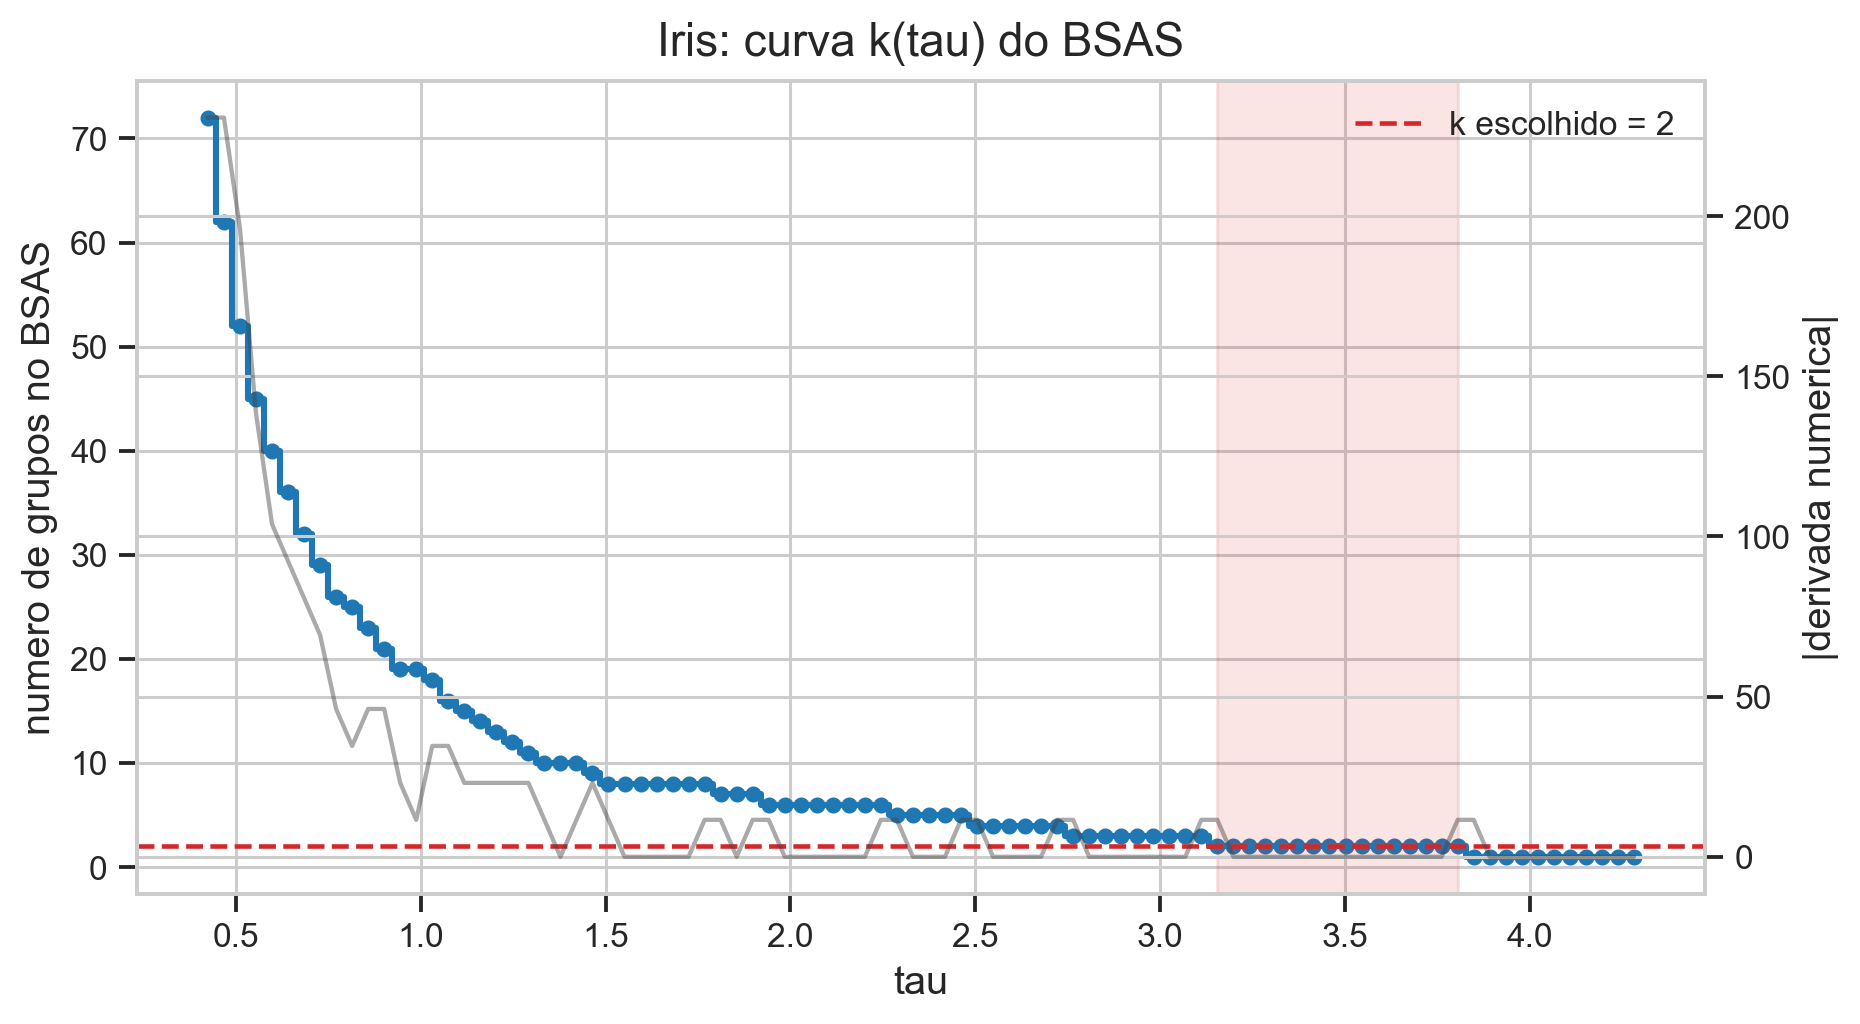
\includegraphics[width=0.82\textwidth]{assets/iris_tau.png}
    \caption{Curva $k(\tau)$ usada para apoiar a escolha do n\'umero de grupos no Iris.}
    \label{fig:iris-tau}
\end{figure}


\begin{figure}[htbp]
    \centering
    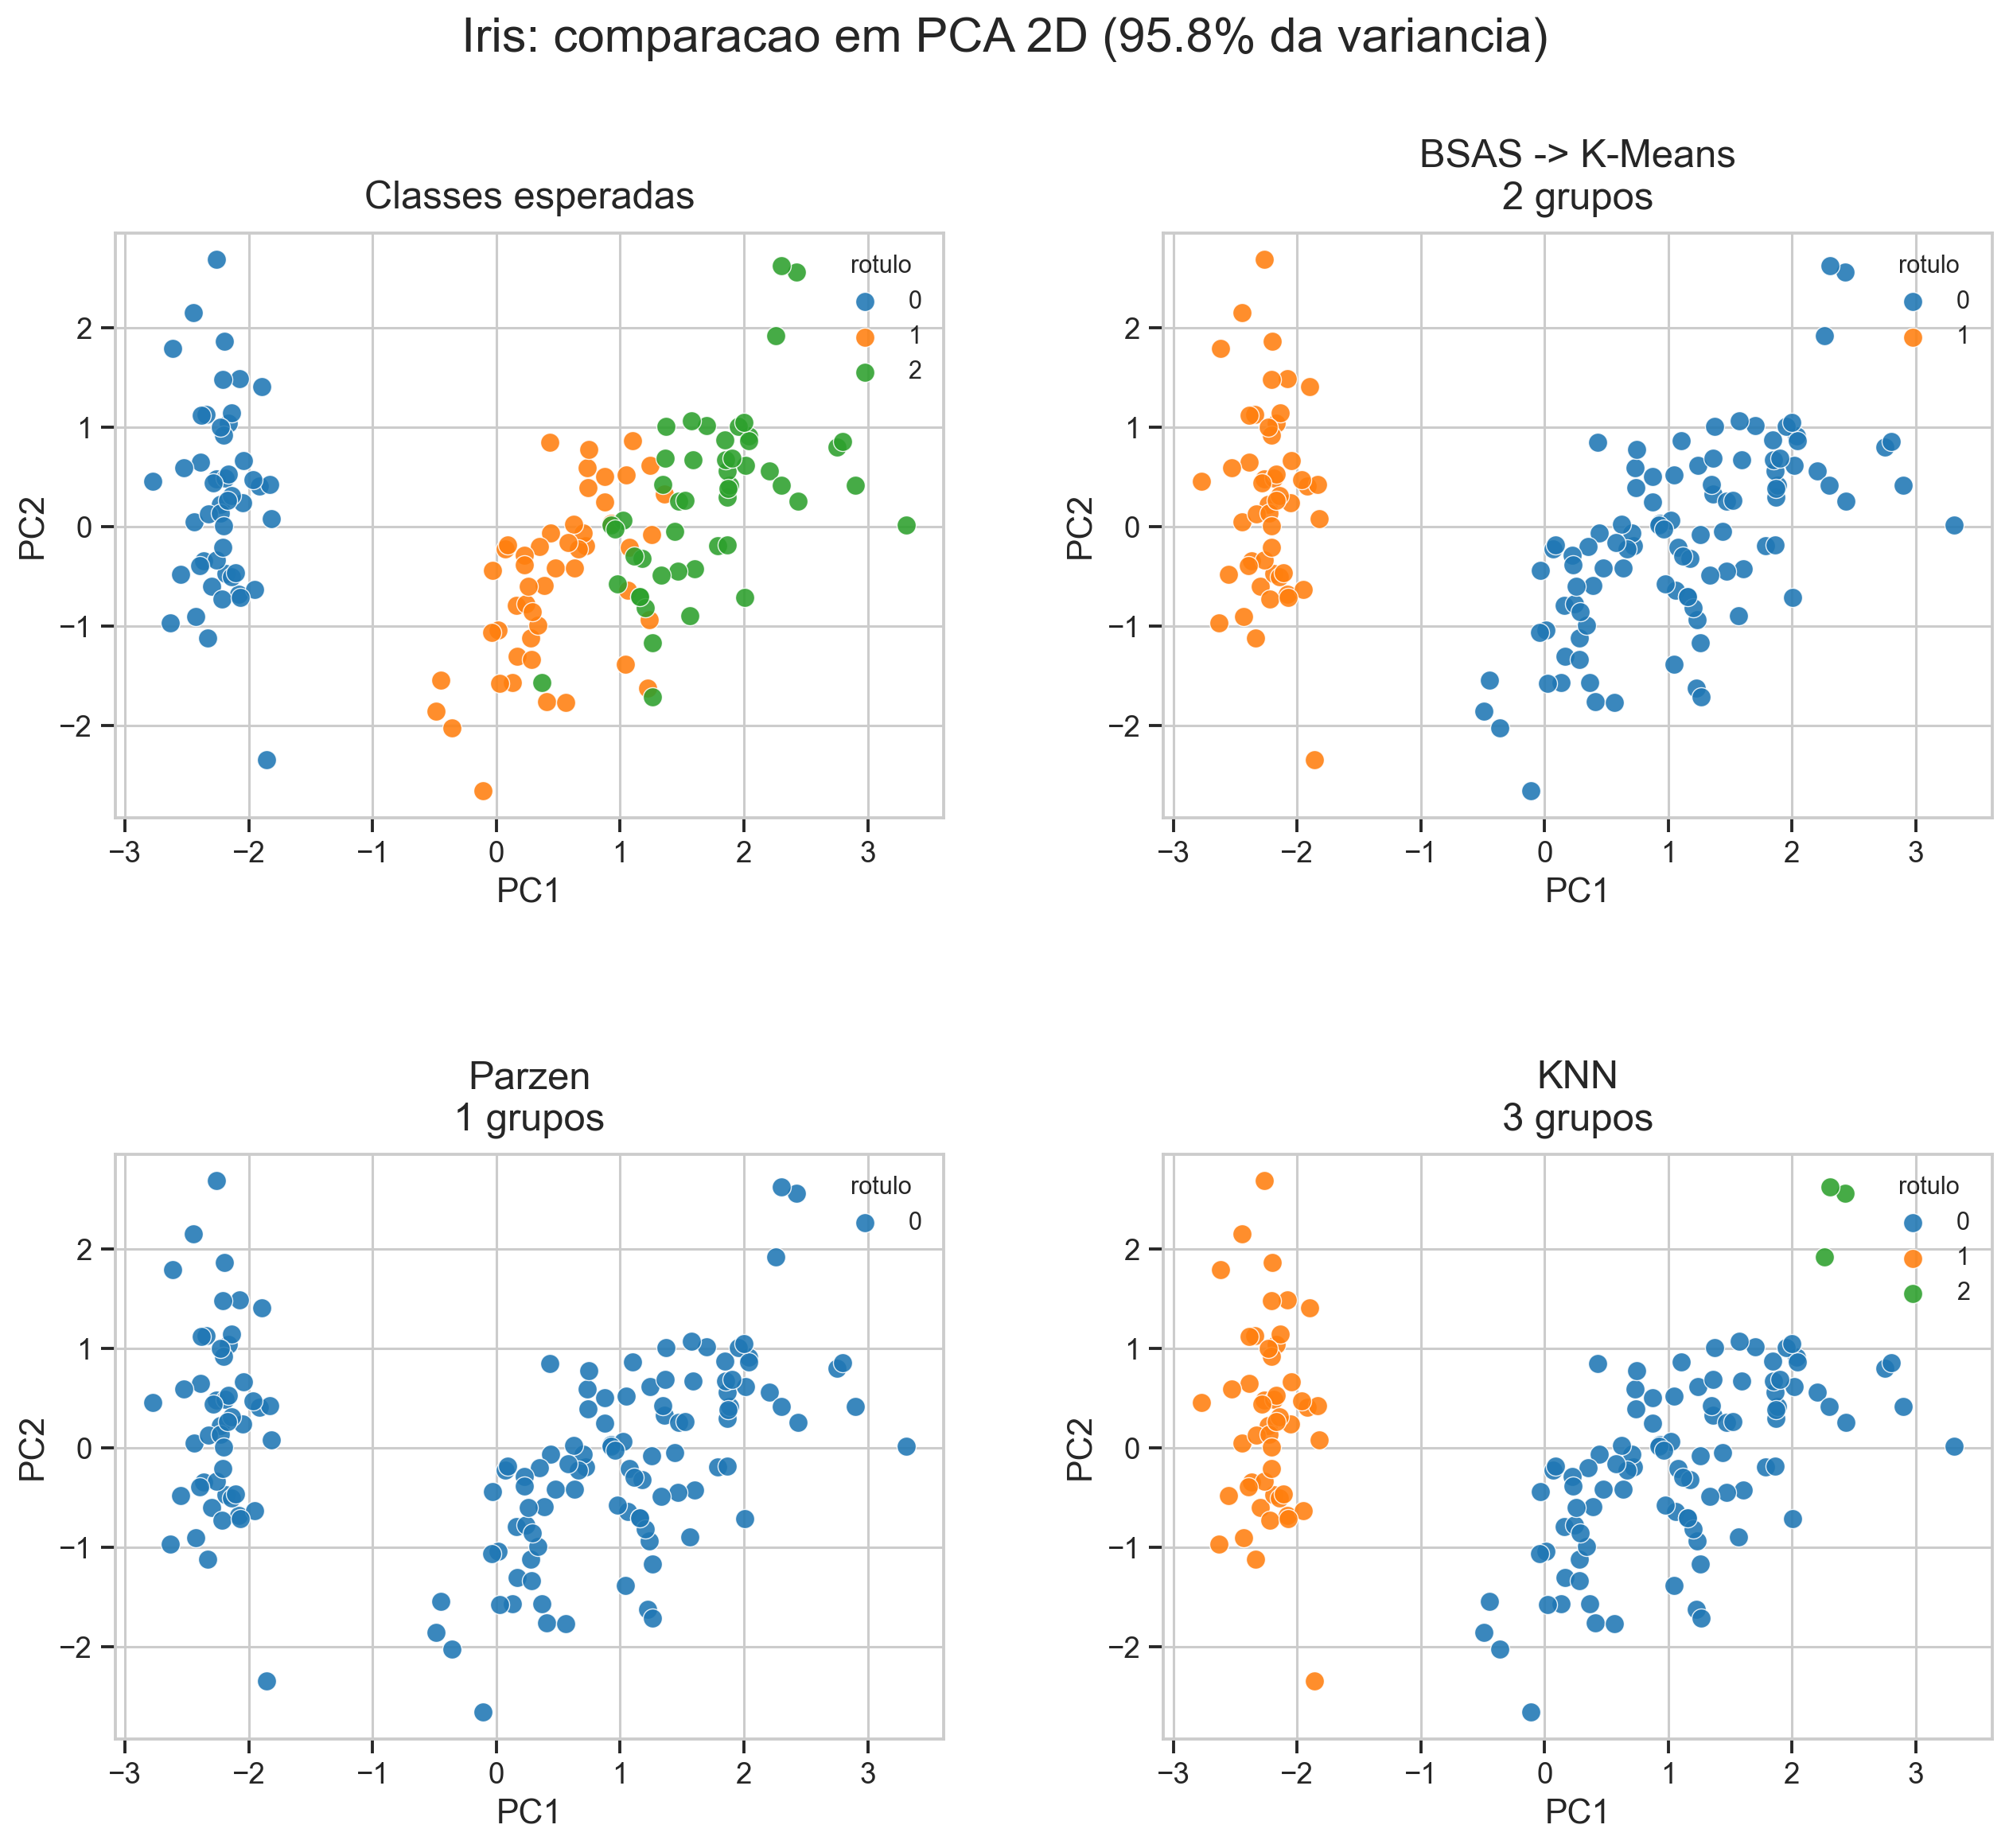
\includegraphics[width=\textwidth]{assets/comparacao_iris_pca.png}
    \caption{Compara\c{c}\~ao qualitativa dos agrupamentos do Iris no plano PCA 2D.}
    \label{fig:comparacao-iris-pca}
\end{figure}


\FloatBarrier


\subsection{Wine Dataset}

No Wine Dataset, a padronização é ainda mais importante, pois os atributos
possuem escalas numéricas muito diferentes. Após esse pré-processamento, a PCA
geralmente evidencia uma separação razoável entre as classes, embora algumas
regiões possam permanecer próximas.

A combinação BSAS e K-Means tende a funcionar bem quando a curva $k(\tau)$
apresenta um plateau associado a um número de grupos compatível com a estrutura
esperada. A vantagem dessa abordagem é a interpretabilidade da escolha de $k$:
o gráfico permite visualizar se o número de grupos foi escolhido em uma região
estável ou em uma transição abrupta.

No caso do Parzen, a escolha da largura da janela tem impacto direto na
resolução da densidade. Como Wine possui mais atributos que Iris, a estimativa
de densidade pode ser mais difícil devido ao aumento da dimensionalidade. Em
dimensões mais altas, os pontos tendem a ficar mais esparsos, o que torna a
escolha do \textit{bandwidth} mais delicada.

O método KNN com vizinhos compartilhados pode capturar estruturas locais
interessantes, principalmente quando os grupos possuem densidades diferentes.
Por outro lado, se $K$ for pequeno demais, o grafo pode se fragmentar em muitas
componentes. Se $K$ for grande demais, regiões distintas podem ser conectadas,
reduzindo a separação entre grupos.

\begin{figure}[htbp]
    \centering
    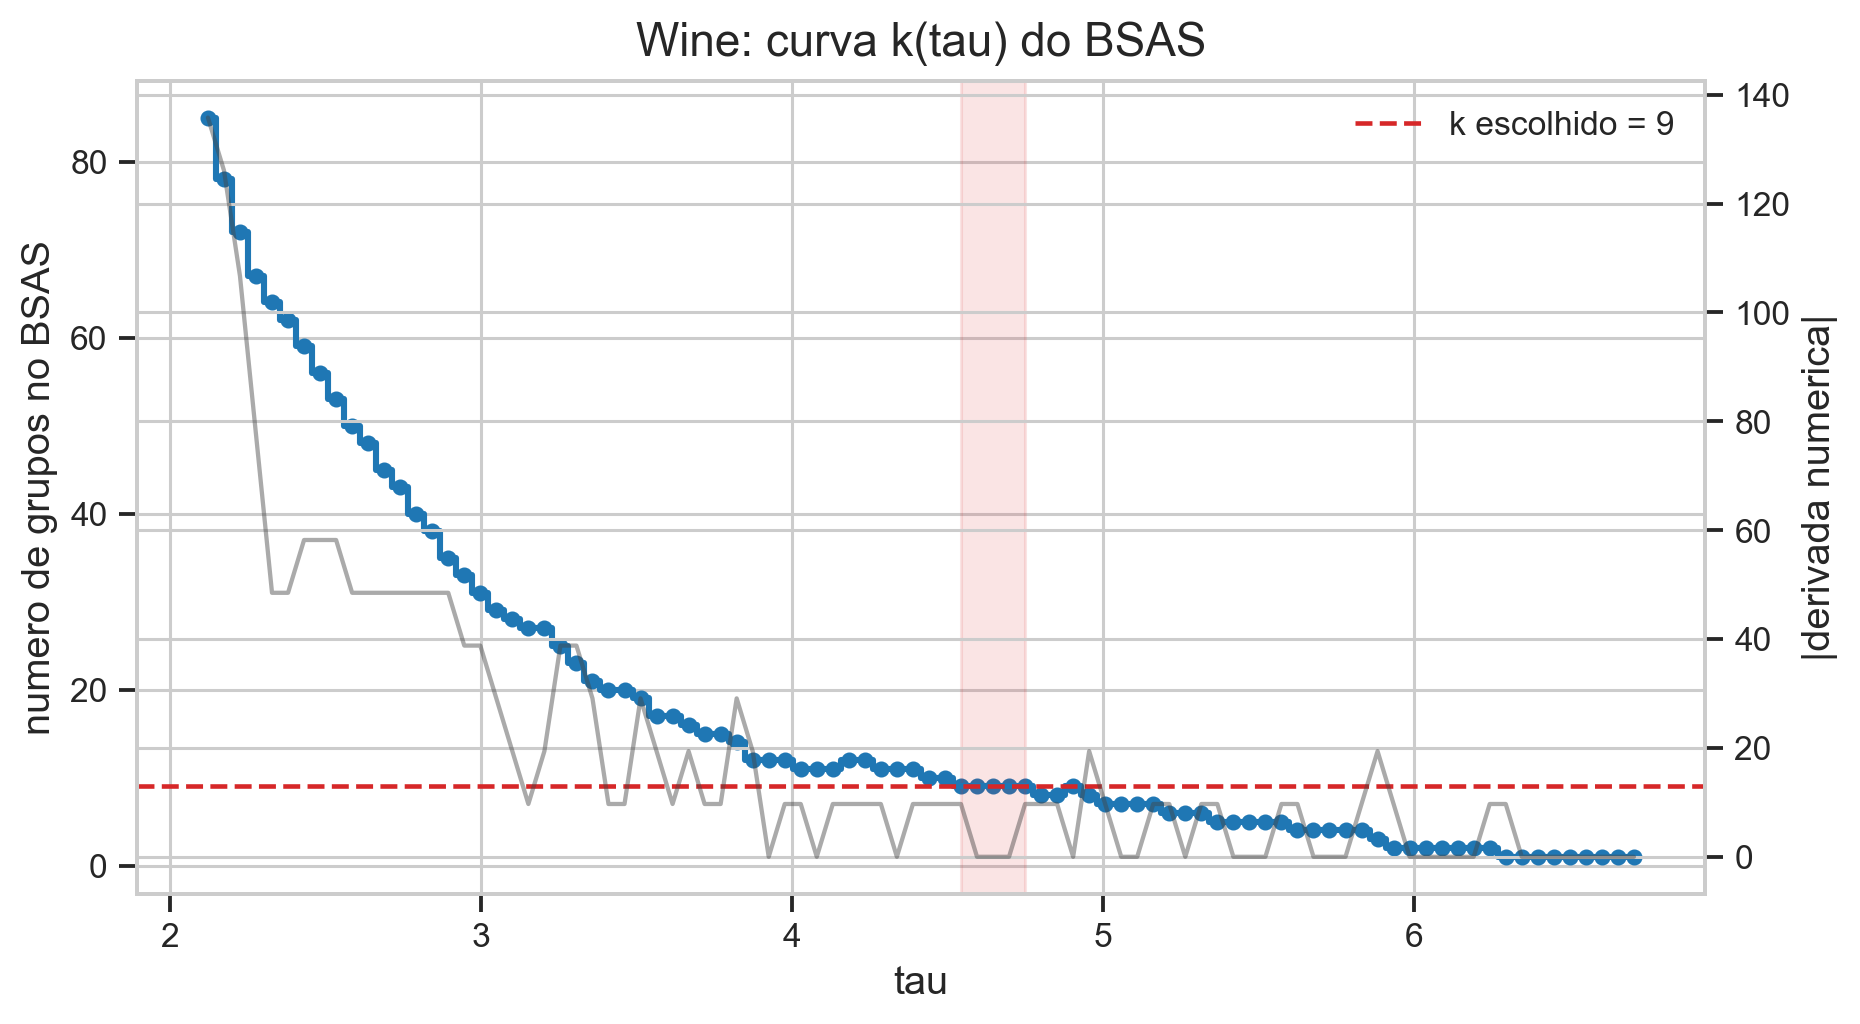
\includegraphics[width=0.82\textwidth]{assets/wine_tau.png}
    \caption{Curva $k(\tau)$ usada para apoiar a escolha do n\'umero de grupos no Wine.}
    \label{fig:wine-tau}
\end{figure}

\begin{figure}[htbp]
    \centering
    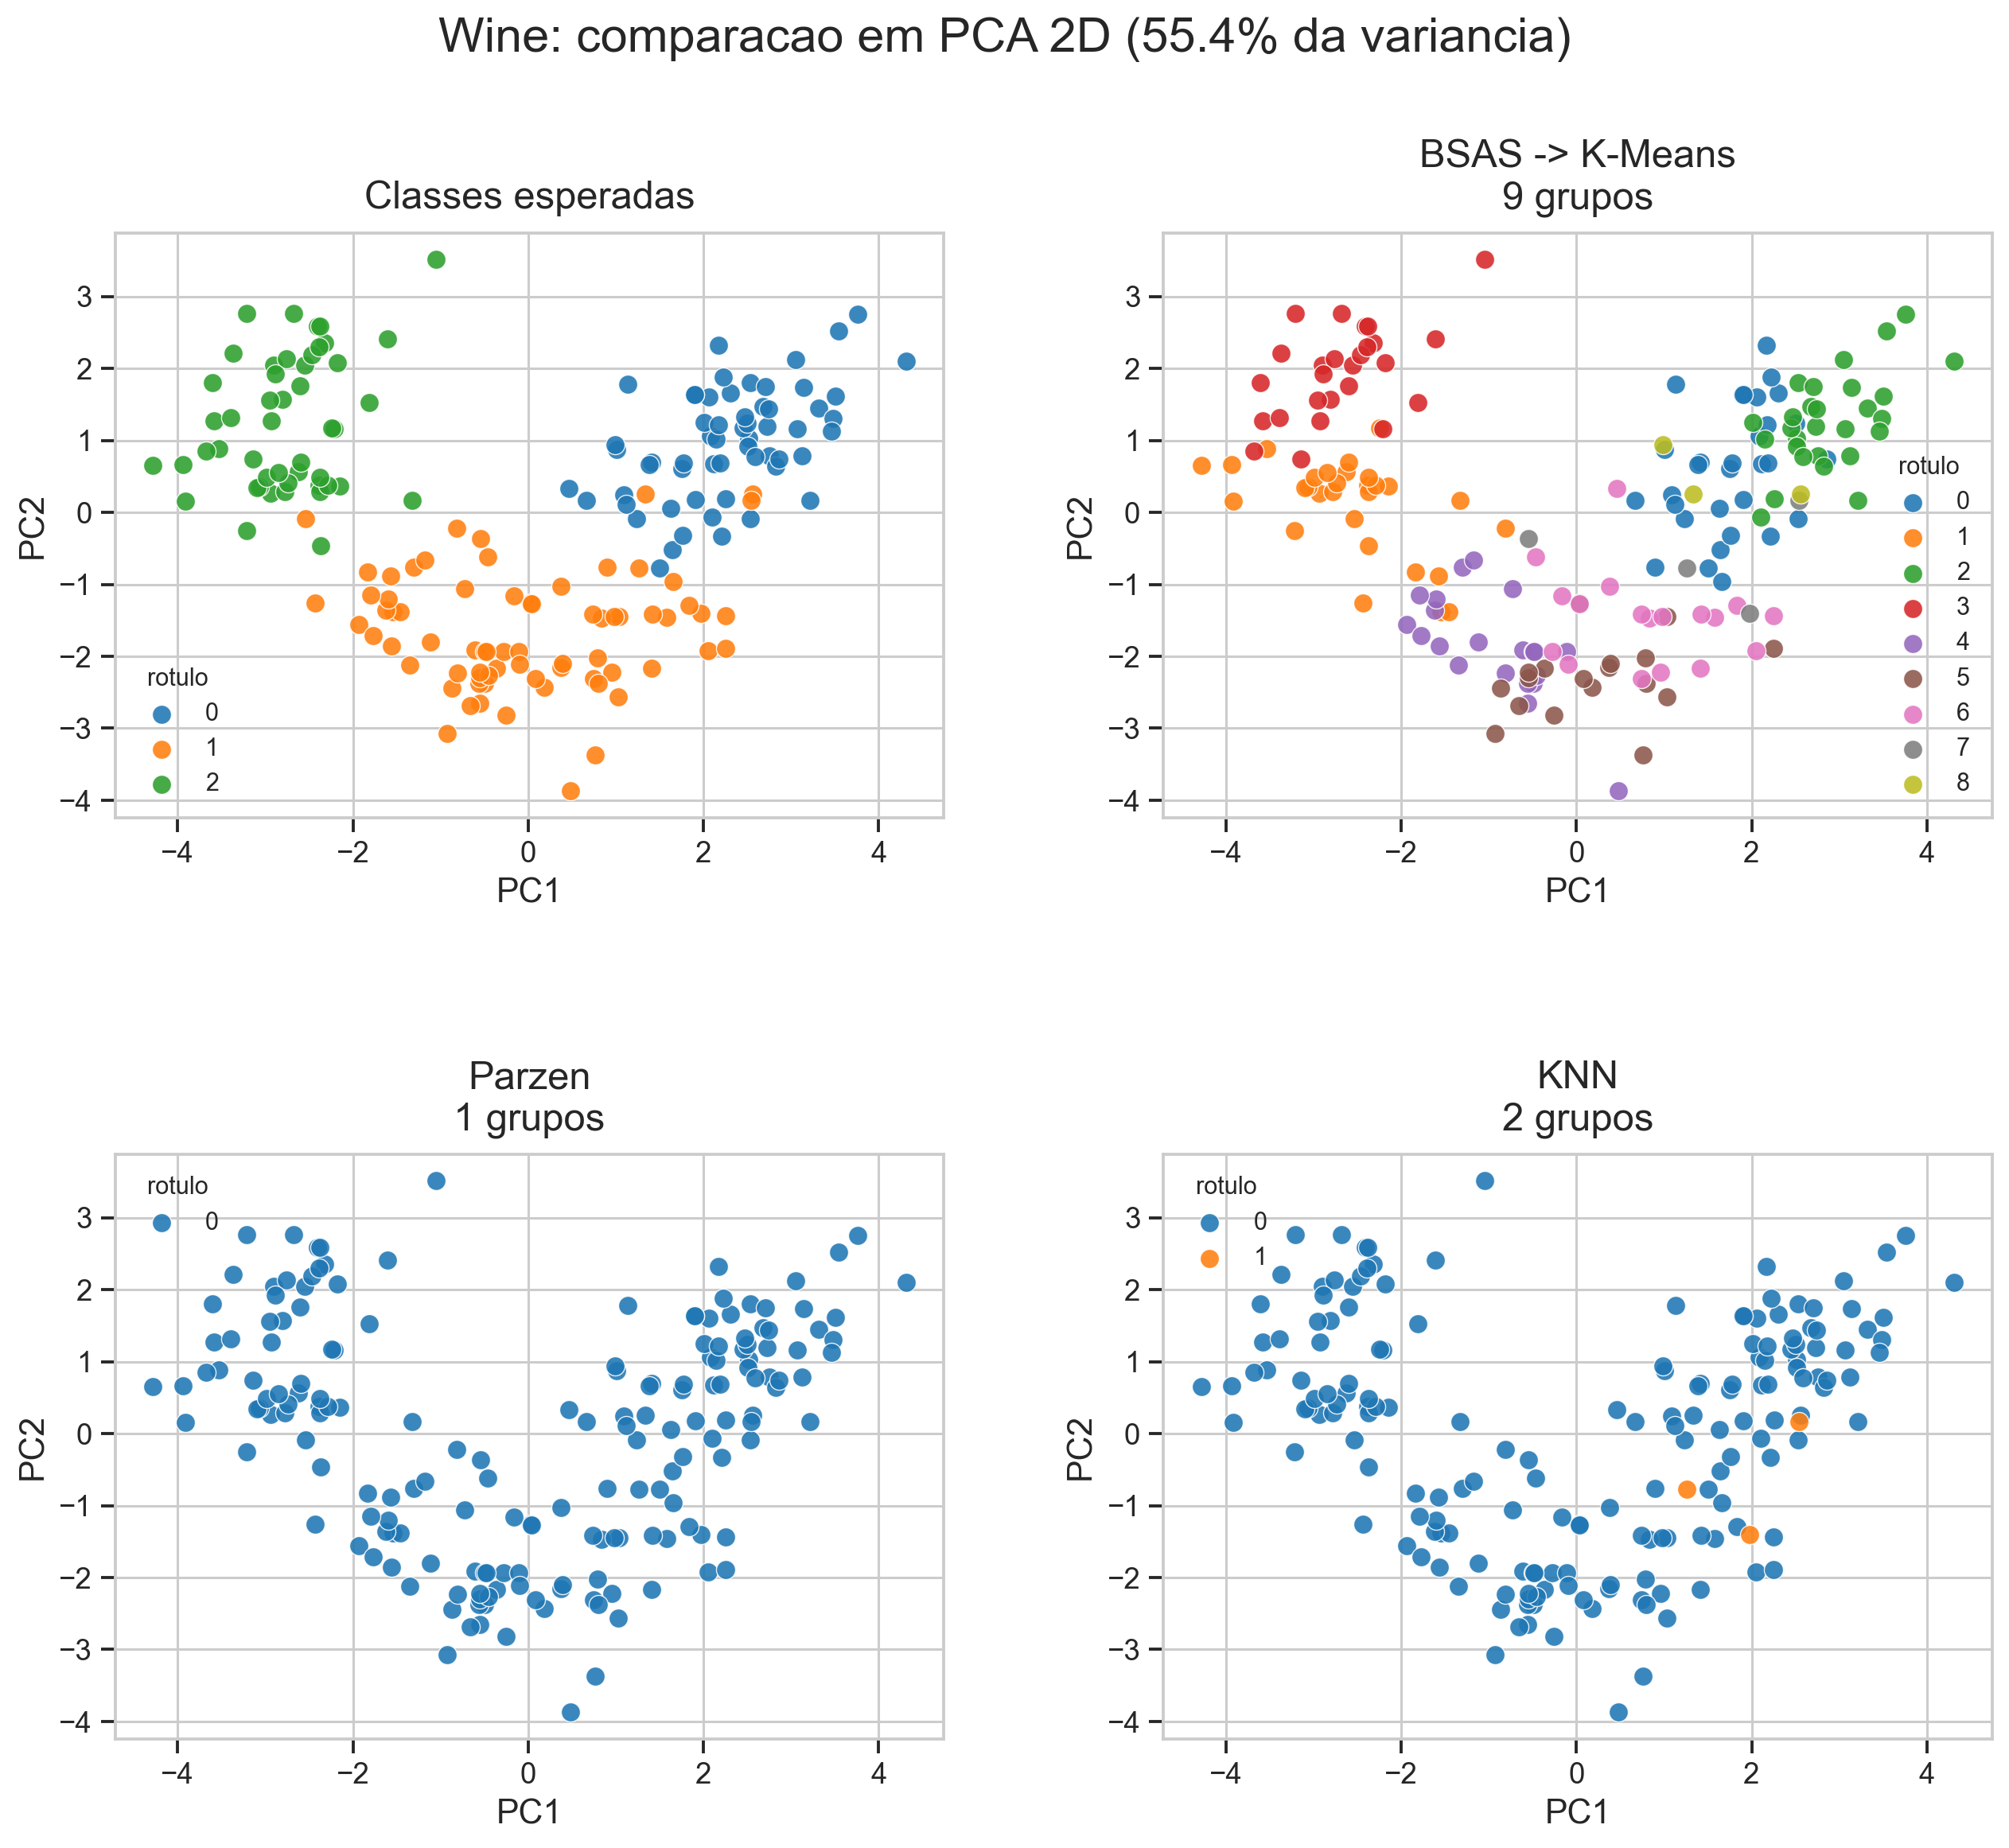
\includegraphics[width=\textwidth]{assets/comparacao_wine_pca.png}
    \caption{Compara\c{c}\~ao qualitativa dos agrupamentos do Wine no plano PCA 2D.}
    \label{fig:comparacao-wine-pca}
\end{figure}

\FloatBarrier

\section{Sensibilidade a parâmetros}

Os três procedimentos possuem parâmetros importantes. A Tabela
\ref{tab:parametros} resume os principais efeitos observados.

\begin{table}[h]
\centering
\caption{Sensibilidade dos métodos aos principais parâmetros.}
\label{tab:parametros}
\begin{tabular}{lll}
\toprule
Metodo & Parâmetro & Efeito principal \\
\midrule
BSAS & $\tau$ & Controla a criação de novos grupos. \\
K-Means & $k$ & Define diretamente o número de clusters finais. \\
Parzen & $h$ & Controla a suavização da densidade estimada. \\
KNN & $K$ & Controla o tamanho da vizinhança local. \\
KNN & vizinhos compartilhados & Controla a rigidez das conexões do grafo. \\
\bottomrule
\end{tabular}
\end{table}

No BSAS, $\tau$ é o parâmetro mais crítico. Valores baixos levam a muitos
clusters; valores altos levam a poucos clusters. A estratégia de observar
plateaus na curva $k(\tau)$ reduz essa arbitrariedade, mas não elimina
completamente a necessidade de julgamento.

No K-Means, o parâmetro $k$ determina o número final de grupos. Por isso, usar o
BSAS como etapa anterior é uma forma de tornar a escolha mais fundamentada.
Ainda assim, se o BSAS estimar um $k$ inadequado, o K-Means herdará essa
limitação.

No Parzen, a largura da janela $h$ controla a suavidade da densidade. Um $h$
muito pequeno gera muitos picos locais e pode fragmentar os dados. Um $h$ muito
grande suaviza demais a densidade e pode unir grupos distintos.

No KNN, $K$ e o número mínimo de vizinhos compartilhados controlam a
conectividade do grafo. Parâmetros muito permissivos criam conexões entre grupos
distintos; parâmetros muito restritivos quebram grupos naturais em várias
componentes pequenas.

\section{Vantagens e desvantagens}

\begin{table}[H]
\centering
\caption{Comparação qualitativa das abordagens implementadas.}
\label{tab:comparacao}
\begin{tabular}{p{3cm}p{5.4cm}p{5.4cm}}
\toprule
Metodo & Vantagens & Desvantagens \\
\midrule
BSAS + K-Means
& Estima automaticamente $k$; possui interpretação visual pela curva
$k(\tau)$; K-Means é simples e eficiente.
& BSAS é sensível à ordem dos dados; K-Means favorece grupos aproximadamente
esféricos; resultado depende do plateau escolhido. \\
\addlinespace
Parzen
& Relaciona agrupamentos a regiões de alta densidade; pode encontrar grupos
sem impor diretamente um valor de $k$; densidade estimada é visualizável.
& Muito sensível ao \textit{bandwidth}; sofre em dimensionalidade alta; pode
fundir ou fragmentar grupos dependendo da suavização. \\
\addlinespace
KNN
& Explora estrutura local; pode lidar melhor com formatos não esféricos; evita
algumas conexões fracas usando vizinhos compartilhados.
& Sensível a $K$ e ao critério de vizinhos compartilhados; pode gerar muitas
componentes pequenas; custo de construir vizinhanças cresce com o número de
amostras. \\
\bottomrule
\end{tabular}
\end{table}

\FloatBarrier

\section{Limitações}

Uma limitação geral é que as visualizações em PCA 2D mostram apenas uma
projeção dos dados. Separações ou sobreposições vistas no gráfico podem não
representar perfeitamente a geometria no espaço original. Portanto, os gráficos
devem ser interpretados como apoio qualitativo, não como prova absoluta da
estrutura dos grupos.

Outra limitação é a dependência de parâmetros. Embora tenham sido usadas regras
automáticas ou semi-automáticas para definir alguns valores, ainda existe
sensibilidade a escolhas como $\tau$, \textit{bandwidth}, $K$ e número mínimo de
vizinhos compartilhados. Uma análise mais completa poderia testar grades de
parâmetros e avaliar a estabilidade dos agrupamentos.

O BSAS também apresenta dependência da ordem dos dados. A implementação reduz
esse problema ao executar múltiplos embaralhamentos e usar a mediana de $k$, mas
isso não remove totalmente a característica sequencial do método.

Por fim, os datasets Iris e Wine são relativamente pequenos e bem conhecidos.
Em bases maiores, com ruído, atributos irrelevantes ou estruturas mais
complexas, o comportamento dos métodos pode ser diferente. Especialmente no
caso de Parzen, a estimativa de densidade pode se tornar mais difícil em
dimensões elevadas.

\section{Conclusão}

A atividade mostrou que diferentes ideias de agrupamento enfatizam aspectos
distintos dos dados. A combinação BSAS + K-Means é uma alternativa útil quando
se deseja estimar o número de clusters antes de aplicar um particionador
clássico. A análise da curva $k(\tau)$ e de sua derivada numérica fornece uma
justificativa visual e quantitativa para a escolha de $k$.

O método baseado em Janelas de Parzen oferece uma interpretação por densidade:
grupos são associados a regiões de maior concentração de pontos. Essa abordagem
é intuitiva e visualmente rica, mas depende fortemente da largura da janela. O
método KNN, por sua vez, modela a estrutura local dos dados por meio de um
grafo, sendo interessante para identificar grupos conectados por vizinhanças
semelhantes.

Em termos práticos, nenhuma abordagem é universalmente superior. BSAS + K-Means
é simples e eficiente, mas assume uma estrutura de grupos mais regular. Parzen é
mais flexível em termos de densidade, mas é sensível à suavização. KNN
captura relações locais, mas depende da conectividade do grafo. Assim, a melhor
interpretação dos resultados surge da combinação entre visualização, métricas de
apoio e análise crítica da sensibilidade dos parâmetros.

\end{document}
